\documentclass{standalone}
\usepackage{tikz}
\usetikzlibrary{patterns, positioning}
\usetikzlibrary{shapes.misc}
\usepackage[outline]{contour}
\contourlength{1.5pt} 
\usepackage[sfdefault]{ClearSans} %% option 'sfdefault' activates Clear Sans as the default text font
\usepackage[T1]{fontenc}

\begin{document}
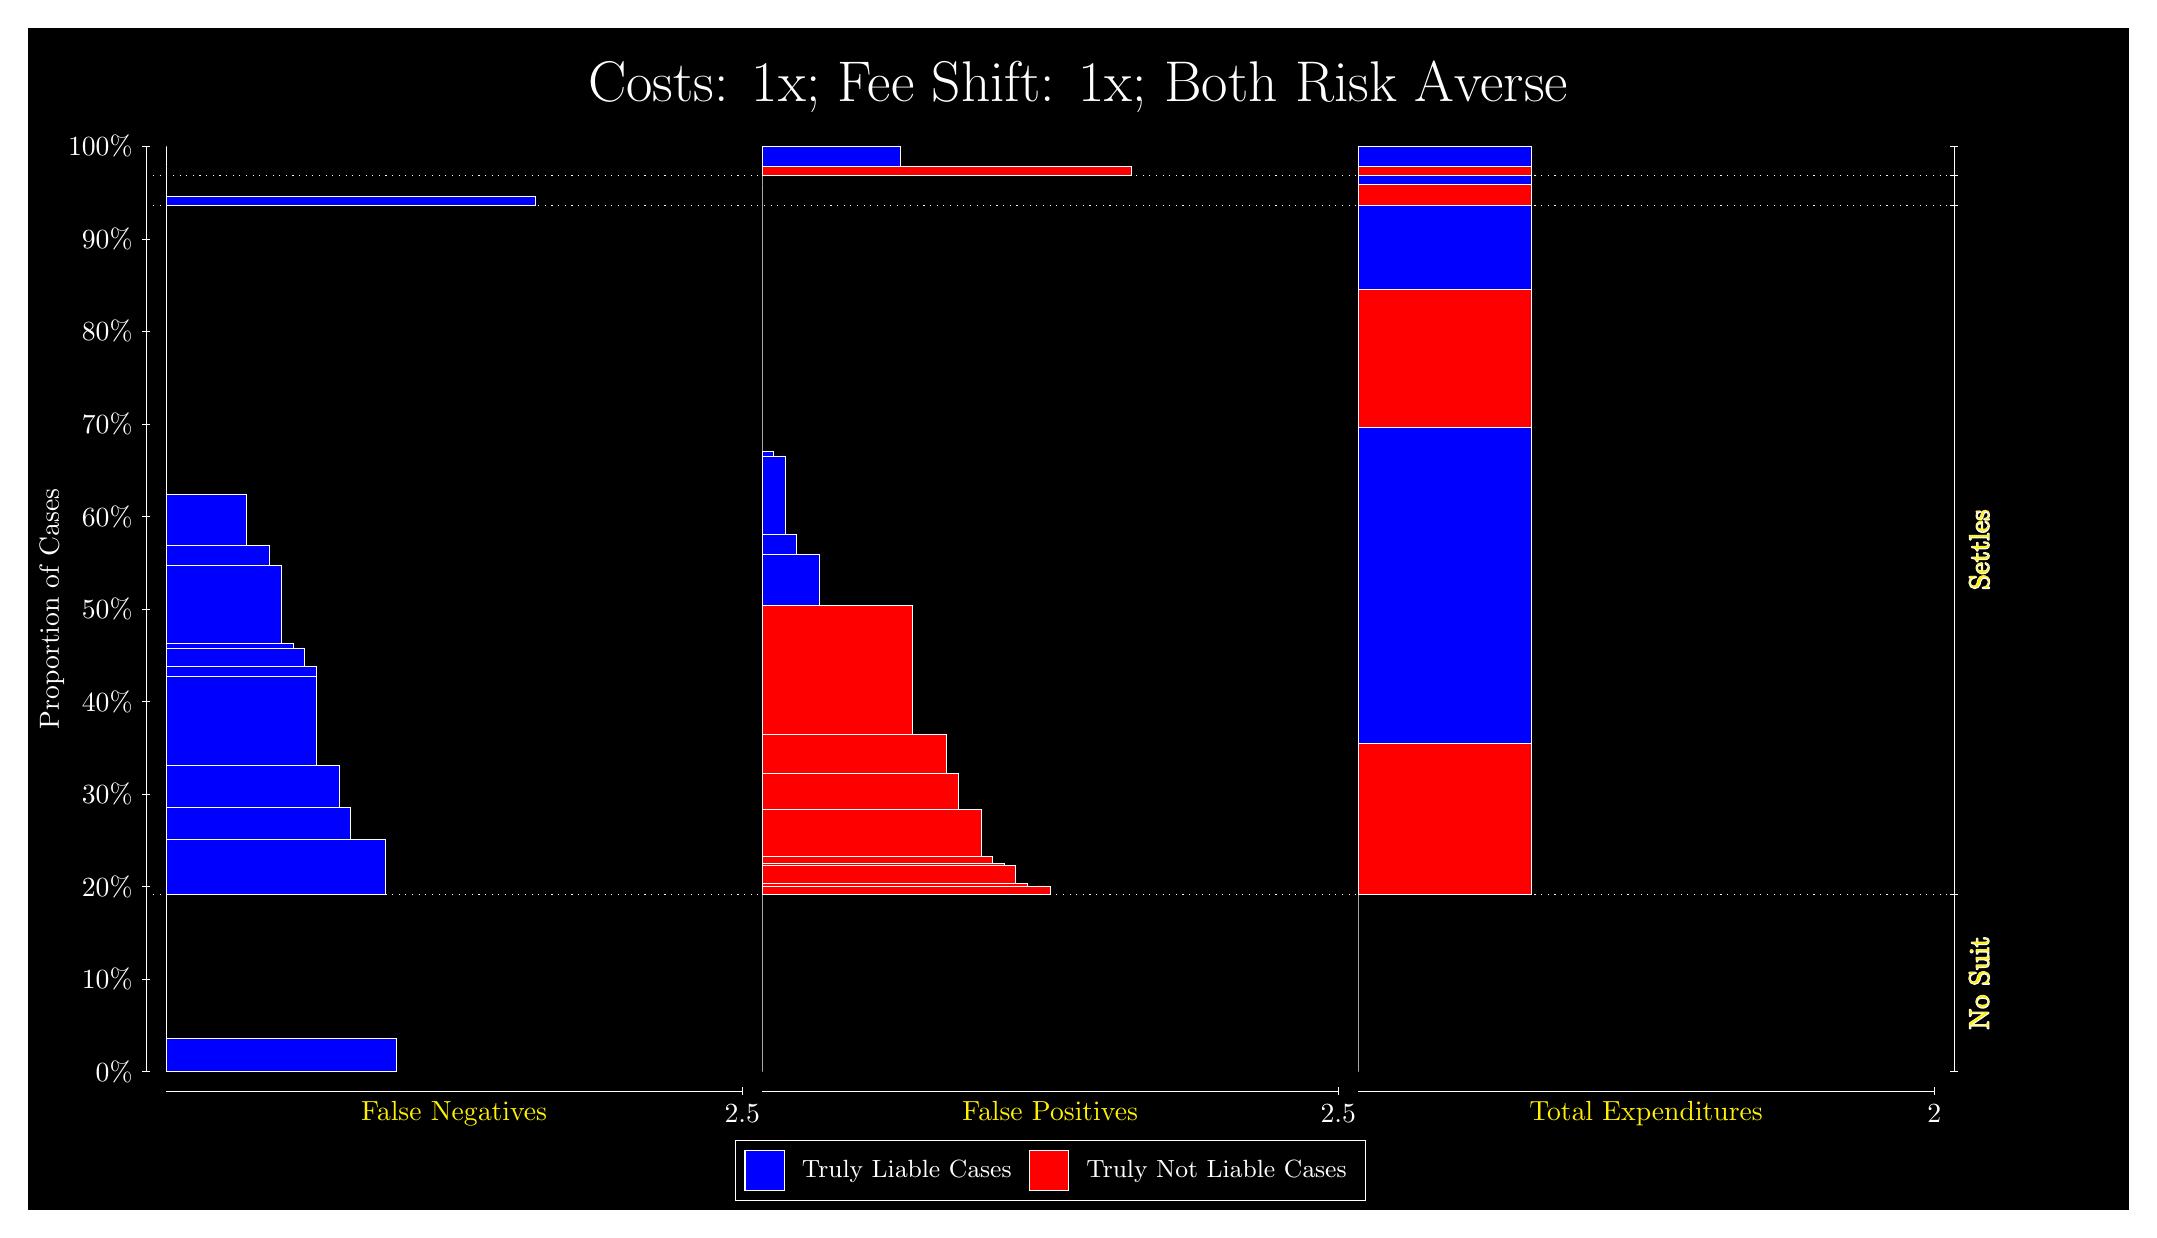
\begin{tikzpicture}
\draw[fill=black] (0,0) rectangle (26.667,15);
\draw[text=white] (0,13.5) rectangle (26.667,15) node[midway] {\huge Costs: 1x; Fee Shift: 1x; Both Risk Averse};
\draw[white, very thin] (1.5,1.75) -- (1.5,13.5);
\node[rotate=90, text=white, anchor=center] at (0.3, 7.625) {Proportion of Cases};
\draw[white, very thin] (1.45,1.75) -- (1.55,1.75);
\node[text=white, anchor=east] at (1.45, 1.75) {0\%};
\draw[white, very thin] (1.45,2.925) -- (1.55,2.925);
\node[text=white, anchor=east] at (1.45, 2.925) {10\%};
\draw[white, very thin] (1.45,4.1) -- (1.55,4.1);
\node[text=white, anchor=east] at (1.45, 4.1) {20\%};
\draw[white, very thin] (1.45,5.275) -- (1.55,5.275);
\node[text=white, anchor=east] at (1.45, 5.275) {30\%};
\draw[white, very thin] (1.45,6.45) -- (1.55,6.45);
\node[text=white, anchor=east] at (1.45, 6.45) {40\%};
\draw[white, very thin] (1.45,7.625) -- (1.55,7.625);
\node[text=white, anchor=east] at (1.45, 7.625) {50\%};
\draw[white, very thin] (1.45,8.8) -- (1.55,8.8);
\node[text=white, anchor=east] at (1.45, 8.8) {60\%};
\draw[white, very thin] (1.45,9.975) -- (1.55,9.975);
\node[text=white, anchor=east] at (1.45, 9.975) {70\%};
\draw[white, very thin] (1.45,11.15) -- (1.55,11.15);
\node[text=white, anchor=east] at (1.45, 11.15) {80\%};
\draw[white, very thin] (1.45,12.325) -- (1.55,12.325);
\node[text=white, anchor=east] at (1.45, 12.325) {90\%};
\draw[white, very thin] (1.45,13.5) -- (1.55,13.5);
\node[text=white, anchor=east] at (1.45, 13.5) {100\%};

\draw[white, very thin] (24.457,1.75) -- (24.457,13.5);
\draw[white, very thin] (24.407,1.75) -- (24.507,1.75);
\node[anchor=west] at (24.407, 1.75) {};
\draw[white, very thin] (24.407,4.0004) -- (24.507,4.0004);
\node[anchor=west] at (24.407, 4.0004) {};
\draw[white, very thin] (24.407,12.752) -- (24.507,12.752);
\node[anchor=west] at (24.407, 12.752) {};
\draw[white, very thin] (24.407,13.126) -- (24.507,13.126);
\node[anchor=west] at (24.407, 13.126) {};
\draw[white, very thin] (24.407,13.5) -- (24.507,13.5);
\node[anchor=west] at (24.407, 13.5) {};

\draw[white, very thin, fill=blue] (1.75,1.75) rectangle (4.6775,2.1747);
\draw[white, very thin, fill=red] (1.75,2.1747) rectangle (1.75,4.0004);
\draw[white, very thin, fill=blue] (1.75,4.0004) rectangle (4.5312,4.703);
\draw[white, very thin, fill=blue] (1.75,4.703) rectangle (4.092,5.1082);
\draw[white, very thin, fill=blue] (1.75,5.1082) rectangle (3.9457,5.638);
\draw[white, very thin, fill=blue] (1.75,5.638) rectangle (3.6529,6.7758);
\draw[white, very thin, fill=blue] (1.75,6.7758) rectangle (3.6529,6.8913);
\draw[white, very thin, fill=blue] (1.75,6.8913) rectangle (3.5065,7.1316);
\draw[white, very thin, fill=blue] (1.75,7.1316) rectangle (3.3602,7.1854);
\draw[white, very thin, fill=blue] (1.75,7.1854) rectangle (3.2138,8.1797);
\draw[white, very thin, fill=blue] (1.75,8.1797) rectangle (3.0674,8.4349);
\draw[white, very thin, fill=blue] (1.75,8.4349) rectangle (2.7746,9.0817);
\draw[white, very thin, fill=red] (1.75,9.0817) rectangle (1.75,12.752);
\draw[white, very thin, fill=blue] (1.75,12.752) rectangle (6.4341,12.863);
\draw[white, very thin, fill=red] (1.75,12.863) rectangle (1.75,13.126);
\draw[white, very thin, fill=red] (1.75,13.126) rectangle (1.75,13.242);
\draw[white, very thin, fill=blue] (1.75,13.242) rectangle (1.75,13.5);
\draw[white, very thin, fill=red] (9.3189,1.75) rectangle (9.3189,3.5757);
\draw[white, very thin, fill=blue] (9.3189,3.5757) rectangle (9.3189,4.0004);
\draw[white, very thin, fill=red] (9.3189,4.0004) rectangle (12.978,4.0978);
\draw[white, very thin, fill=red] (9.3189,4.0978) rectangle (12.686,4.1464);
\draw[white, very thin, fill=red] (9.3189,4.1464) rectangle (12.539,4.3708);
\draw[white, very thin, fill=red] (9.3189,4.3708) rectangle (12.393,4.3888);
\draw[white, very thin, fill=red] (9.3189,4.3888) rectangle (12.246,4.4852);
\draw[white, very thin, fill=red] (9.3189,4.4852) rectangle (12.1,5.0836);
\draw[white, very thin, fill=red] (9.3189,5.0836) rectangle (11.807,5.5372);
\draw[white, very thin, fill=red] (9.3189,5.5372) rectangle (11.661,6.0334);
\draw[white, very thin, fill=red] (9.3189,6.0334) rectangle (11.222,7.6709);
\draw[white, very thin, fill=blue] (9.3189,7.6709) rectangle (10.051,8.3177);
\draw[white, very thin, fill=blue] (9.3189,8.3177) rectangle (9.758,8.5729);
\draw[white, very thin, fill=blue] (9.3189,8.5729) rectangle (9.6116,9.5673);
\draw[white, very thin, fill=blue] (9.3189,9.5673) rectangle (9.4652,9.6211);
\draw[white, very thin, fill=blue] (9.3189,9.6211) rectangle (9.3189,12.752);
\draw[white, very thin, fill=red] (9.3189,12.752) rectangle (9.3189,13.015);
\draw[white, very thin, fill=blue] (9.3189,13.015) rectangle (9.3189,13.126);
\draw[white, very thin, fill=red] (9.3189,13.126) rectangle (14.003,13.242);
\draw[white, very thin, fill=blue] (9.3189,13.242) rectangle (11.075,13.5);
\draw[white, very thin, fill=red] (16.888,1.75) rectangle (16.888,3.5757);
\draw[white, very thin, fill=blue] (16.888,3.5757) rectangle (16.888,4.0004);
\draw[white, very thin, fill=red] (16.888,4.0004) rectangle (19.083,5.9207);
\draw[white, very thin, fill=blue] (16.888,5.9207) rectangle (19.083,9.9287);
\draw[white, very thin, fill=red] (16.888,9.9287) rectangle (19.083,11.679);
\draw[white, very thin, fill=blue] (16.888,11.679) rectangle (19.083,12.752);
\draw[white, very thin, fill=red] (16.888,12.752) rectangle (19.083,13.015);
\draw[white, very thin, fill=blue] (16.888,13.015) rectangle (19.083,13.126);
\draw[white, very thin, fill=red] (16.888,13.126) rectangle (19.083,13.242);
\draw[white, very thin, fill=blue] (16.888,13.242) rectangle (19.083,13.5);
\draw[white, dotted] (1.5,4.0004) -- (24.457,4.0004);
\draw[white, dotted] (1.5,12.752) -- (24.457,12.752);
\draw[white, dotted] (1.5,13.126) -- (24.457,13.126);
\draw[white, very thin] (1.75,1.5) -- (9.0689,1.5);
\node[text=yellow, anchor=north] at (5.4094, 1.5) {False Negatives};
\draw[white, very thin] (9.0689,1.45) -- (9.0689,1.55);
\node[text=white, anchor=north] at (9.0689, 1.45) {2.5};

\draw[white, very thin] (9.3189,1.5) -- (16.638,1.5);
\node[text=yellow, anchor=north] at (12.978, 1.5) {False Positives};
\draw[white, very thin] (16.638,1.45) -- (16.638,1.55);
\node[text=white, anchor=north] at (16.638, 1.45) {2.5};

\draw[white, very thin] (16.888,1.5) -- (24.207,1.5);
\node[text=yellow, anchor=north] at (20.547, 1.5) {Total Expenditures};
\draw[white, very thin] (24.207,1.45) -- (24.207,1.55);
\node[text=white, anchor=north] at (24.207, 1.45) {2};

\node[text=yellow, centered, rotate=90] at (24.777, 2.8752) {\contour{white}{No Suit}};
\node[text=yellow, centered, rotate=90] at (24.777, 8.3763) {\contour{white}{Settles}};



\draw (12.978300999999998,1.5) node[draw=none] (baseCoordinate) {};
\begin{scope}[align=center]
        \matrix[scale=0.5, draw=white, below=0.5cm of baseCoordinate, nodes={draw}, column sep=0.1cm]{
            \node[rectangle, draw, minimum width=0.5cm, minimum height=0.5cm, fill=blue] {}; &
            \node[draw=none, font=\small, text=white] (B) {Truly Liable Cases}; &
            \node[rectangle, draw, minimum width=0.5cm, minimum height=0.5cm, fill=red] {}; &
            \node[draw=none, font=\small, text=white] (B) {Truly Not Liable Cases}; \\
            };
\end{scope}

\end{tikzpicture}
\end{document}